%  This LaTeX template is based on T.J. Hitchman's work which is itself based on Dana Ernst's template.  
% 
% --------------------------------------------------------------
% Skip this stuff, and head down to where it says "Start here"
% --------------------------------------------------------------
 
\documentclass[12pt]{article}
\usepackage{subcaption}

\usepackage[margin=1in]{geometry} 
\usepackage{amsmath,amsthm,amssymb}
\usepackage{graphicx}
\newenvironment{statement}[2][Statement]{\begin{trivlist}
\item[\hskip \labelsep {\bfseries #1}\hskip \labelsep {\bfseries #2.}]}{\end{trivlist}}

\begin{document}
 
% --------------------------------------------------------------
%
%                         Start here
%
% --------------------------------------------------------------
 
\title{Circle packing for bp, hp, and 22.5} % replace with the problem you are writing up
\author{Brandon Wong} % replace with your name
\maketitle
Packing in uniaxial origami design can be formalized as a constrained non-linear optimization problem. In a tree with $n$ nodes, we are finding the point in $2n+1$ dimensional space (2 dimensions for the $x$ and $y$ coordinates of each node, and 1 dimension for the scale) that minimizes some objective function while satisfying some constraints. If the objective function (typically, the negative of the scale, to maximize efficiency) and constraint equations are all continuous and differentiable, then we can throw them into an optimization library and obtain a locally optimal packing. Robert Lang's treeMaker software does this for circle packing, now we would like to similarly automate packing in bp, hp, and 22.5. We will leave cp construction as a problem for later.

\section{Non-overlap constraint equations}
Consider the path between two nodes $u_i,u_j$.  Let $L$ be the length of the traversal path between the two nodes on the tree, $\sigma$ be the scale, and let $\Delta x = u_{i_x} - u_{j_x}$ and $\Delta y = u_{i_y} - u_{j_y}$. In circle packing, it is known that the constraint equation to prevent overlaps is simply:
\begin{equation}\label{eq:circle}
    \sqrt{\Delta x^2 + \Delta y^2}-L\sigma \geq 0
\end{equation}
\subsection{Bp}
To pack squares that don't overlap, the constraint becomes non-differentiable:
\[
    \max(\left| \Delta x\right|, \left|\Delta y\right|) - L\sigma \geq 0
\]
We can rewrite this as the maximum dot product of the vector $\begin{bmatrix}
        \Delta x\\
        \Delta y
    \end{bmatrix}$ with the unit basis vectors $\hat e_1= \begin{bmatrix}1\\0\end{bmatrix}$ and $\hat e_2= \begin{bmatrix}0\\1\end{bmatrix}$, as well as their negatives $\hat e_3= \begin{bmatrix}-1\\0\end{bmatrix}$ and $\hat e_4= \begin{bmatrix}0\\-1\end{bmatrix}$:
\[
    \max(\hat e_1^T\begin{bmatrix}
        \Delta x\\
        \Delta y
    \end{bmatrix}, \hat e_2^T\begin{bmatrix}
        \Delta x\\
        \Delta y
    \end{bmatrix}, \hat e_3^T\begin{bmatrix}
        \Delta x\\
        \Delta y
    \end{bmatrix}, \hat e_4^T\begin{bmatrix}
        \Delta x\\
        \Delta y
    \end{bmatrix}) - L\sigma \geq 0
\]
Then, to approximate the function as differentiable, we can approximate the max function with a smooth max function defined as:
\begin{equation}\label{eq:max}
    \max(x_1,x_2,\ldots x_n) \approx \frac{\ln\left[\sum_{i=1}^{n} e^{\alpha x_i}\right]}{\alpha}
\end{equation}
which will approach the true max function as the hyperparameter $\alpha$ approaches infinity. Fully expanded, this looks like:
\begin{equation}\label{eq:bp full}
    \frac{1}{\alpha}\ln\left[e^{\alpha \begin{bmatrix}1 & 0\end{bmatrix}\begin{bmatrix}
        \Delta x\\
        \Delta y
        \end{bmatrix}} + e^{\alpha \begin{bmatrix}0 & 1\end{bmatrix}\begin{bmatrix}
        \Delta x\\
        \Delta y
        \end{bmatrix}} + e^{\alpha \begin{bmatrix}-1 & 0\end{bmatrix}\begin{bmatrix}
        \Delta x\\
        \Delta y
        \end{bmatrix}} + e^{\alpha \begin{bmatrix}0 & -1\end{bmatrix}\begin{bmatrix}
        \Delta x\\
        \Delta y
        \end{bmatrix}}\right]\ - L\sigma \geq 0 
\end{equation}
If we are ok with pythagorean stretches, we'll use the constraint equation from circle packing (\ref{eq:circle}) but will use bp-specific objective functions.

\subsection{Hp}
A similar constraint equation can be derived for packing non-overlapping hexagons and octagons simply by changing the set of basis vectors. In hp, they are as follows:
\[
\{
    \begin{bmatrix}1\\0\end{bmatrix},
    \begin{bmatrix}\frac{1}{2}\\\frac{\sqrt{3}}{2}\end{bmatrix},
    \begin{bmatrix}-\frac{1}{2}\\\frac{\sqrt{3}}{2}\end{bmatrix},
    \begin{bmatrix}-1\\0\end{bmatrix},
    \begin{bmatrix}-\frac{1}{2}\\-\frac{\sqrt{3}}{2}\end{bmatrix},
    \begin{bmatrix}\frac{1}{2}\\-\frac{\sqrt{3}}{2}\end{bmatrix}
\}
\]
\subsection{22.5}
The same can be done for 22.5, as follows:
\[
\{
    \begin{bmatrix}1\\0\end{bmatrix},
    \begin{bmatrix}\frac{\sqrt{2}}{2}\\\frac{\sqrt{2}}{2}\end{bmatrix},
    \begin{bmatrix}0\\1\end{bmatrix},
    \begin{bmatrix}-\frac{\sqrt{2}}{2}\\\frac{\sqrt{2}}{2}\end{bmatrix},
    \begin{bmatrix}-1\\0\end{bmatrix},
    \begin{bmatrix}-\frac{\sqrt{2}}{2}\\-\frac{\sqrt{2}}{2}\end{bmatrix},
    \begin{bmatrix}0\\-1\end{bmatrix},
    \begin{bmatrix}\frac{\sqrt{2}}{2}\\-\frac{\sqrt{2}}{2}\end{bmatrix}
\}
\]
In 22.5 specifically, which doesn't use pleats, an additional constraint we might like to have is that active paths lie along 45 degree axial lines. We can achieve this with a polar function that has the minimum values of $r$ only when $\theta$ is a multiple of $\frac{\pi}{4}$:
\[
    r \geq L\sigma \left[b+1-b\cos(4\theta)^{2k}\right]
\]
See figure~\ref{fig:octagons}. Or in cartesian form:
\begin{equation}\label{eq:polar}
    \sqrt{\Delta x^2 + \Delta y^2} - L\sigma \left[b+1-b\cos(4\arctan(\frac{\Delta y}{\Delta x}))^{2k}\right] \geq 0
\end{equation}
This equation has two hyperparameters $b$ and $k$. $b$ is effectively how far away the flaps should be if being at 45 degrees is not possible---for example, consider two flaps on opposite ends of the cp with many flaps in between them, in which case it doesn't matter whether these flaps are at 45 degrees or not. $k$ is how sharp the function is---the higher $k$ is, the more the function will approach a step function. Additionally, this set of $\Delta x, \Delta y$ that satisfies~(\ref{eq:polar}) is a subset of what would satisfy~(\ref{eq:max}), so it suffices to only use~(\ref{eq:polar}).

\begin{figure}[h]
    \centering
    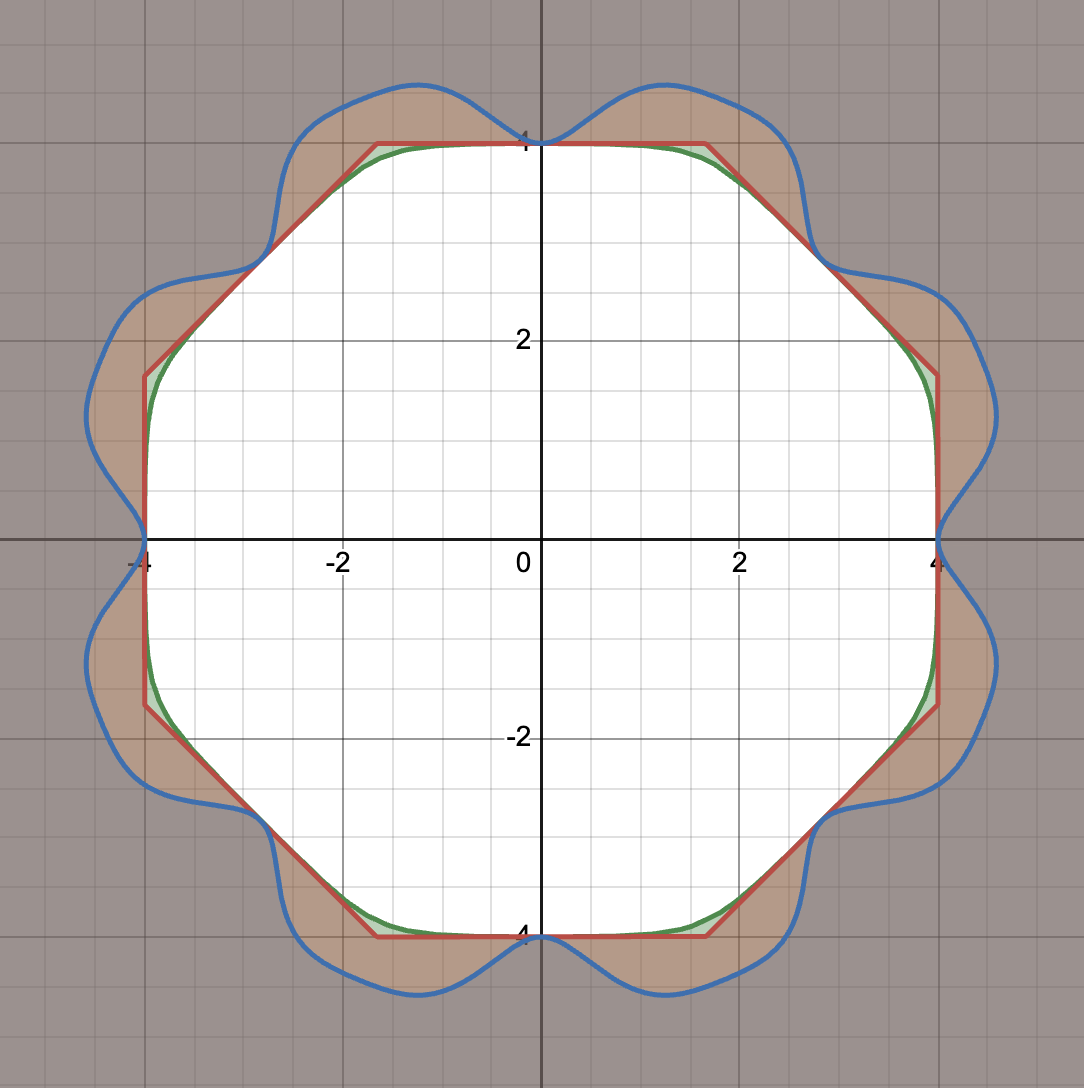
\includegraphics[width=0.7\textwidth]{octagons.png}\caption{A plot of the various possible 22.5 constraint equations for a path of length 4. Orange region: the constraint equation using the true max function. Green region: the constraint equation using the smooth max function with $\alpha=5$. Blue region: the constraint equation using the polar function that constrains active paths to 45 degree axial lines, with $k=1$ and $b=0.2$.}\label{fig:octagons}
\end{figure}

\section{Objective function}
In circle packing, the objective function is simply the negative of the scale to maximize efficiency. However, in bp, hp, and 22.5, we also care about the foldability of the model. In bp and hp, that means that vertices should lie on grid points, and in 22.5, vertice should have easy references (which is itself a challenge to quantify).

\subsection{Bp}
In bp, the objective is not only to maximize the scale, but also that the inverse of the scale (ie, the grid size) is an integer. We could add a constraint equation like:
\[
    \cos^2(\frac{\pi}{\sigma}) - 1 = 0
\]
to constrain the scale to integer grid sizes. However, the allowable values of $\sigma$ would not be continuous, so we must instead put it in the objective function such that it both maximizes the scale as well as maximizes the periodic function:
\[
    -\sigma \left[C_1+\cos^2(\frac{\pi}{\sigma})\right]
\]
This does not guarantee that the grid size will be an integer, but the optimizer will do its best. We use the hyperparameter $C_1$ to control the relative importance of the two terms. When $C_1$ is large, the periodic function still only varies within $[0,1]$, so will be less important for the solver to optimize. There may be some ``sweet spot'' for the hyperparameters that we can find through experimentation and then hard code, or it could be part of the search space, or maybe it's better left a user input.

Next, we want all vertices to lie on grid points. We can include a term with a similar periodic function and prioritization hyperparameter $C_2$ as follows: 
\begin{equation}\label{eq:bp obj}
    -\sigma \left[C_1+\cos^2(\frac{\pi}{\sigma})\right]
    \left[C_2+\sum_{1}^{n}\cos^2(\frac{\pi u_{i_x}}{\sigma}) + \cos^2(\frac{\pi u_{i_y}}{\sigma})\right]
\end{equation}
There are definitely other ways to formulate this equation, for example taking the product of all the vertices rather than the sum. It remains to be seen what's the best way to do this.

\subsection{Hp}
Hex pleating is essentially the same as bp, except instead of the grid size being $\frac{1}{\sigma}$, it is $\frac{2}{\sigma \sqrt{3}}$. We also slightly modify the grid equation to place the vertices onto the hex grid. The objective function is then:
\begin{equation}\label{eq:hp obj}
    -\sigma \left[C_1+\cos^2(\frac{2\pi}{\sigma\sqrt{3}})\right]
    \left[C_2+\sum_{1}^{n}\left[\cos(
        \frac{\pi}{\sigma}(u_{i_y}+\frac{u_{i_x}}{\sqrt{3}})
    ) \cos(
        \frac{\pi}{\sigma}(u_{i_y}-\frac{u_{i_x}}{\sqrt{3}})
    )\right]^2\right]
\end{equation}
\begin{figure}[h]
    \centering
    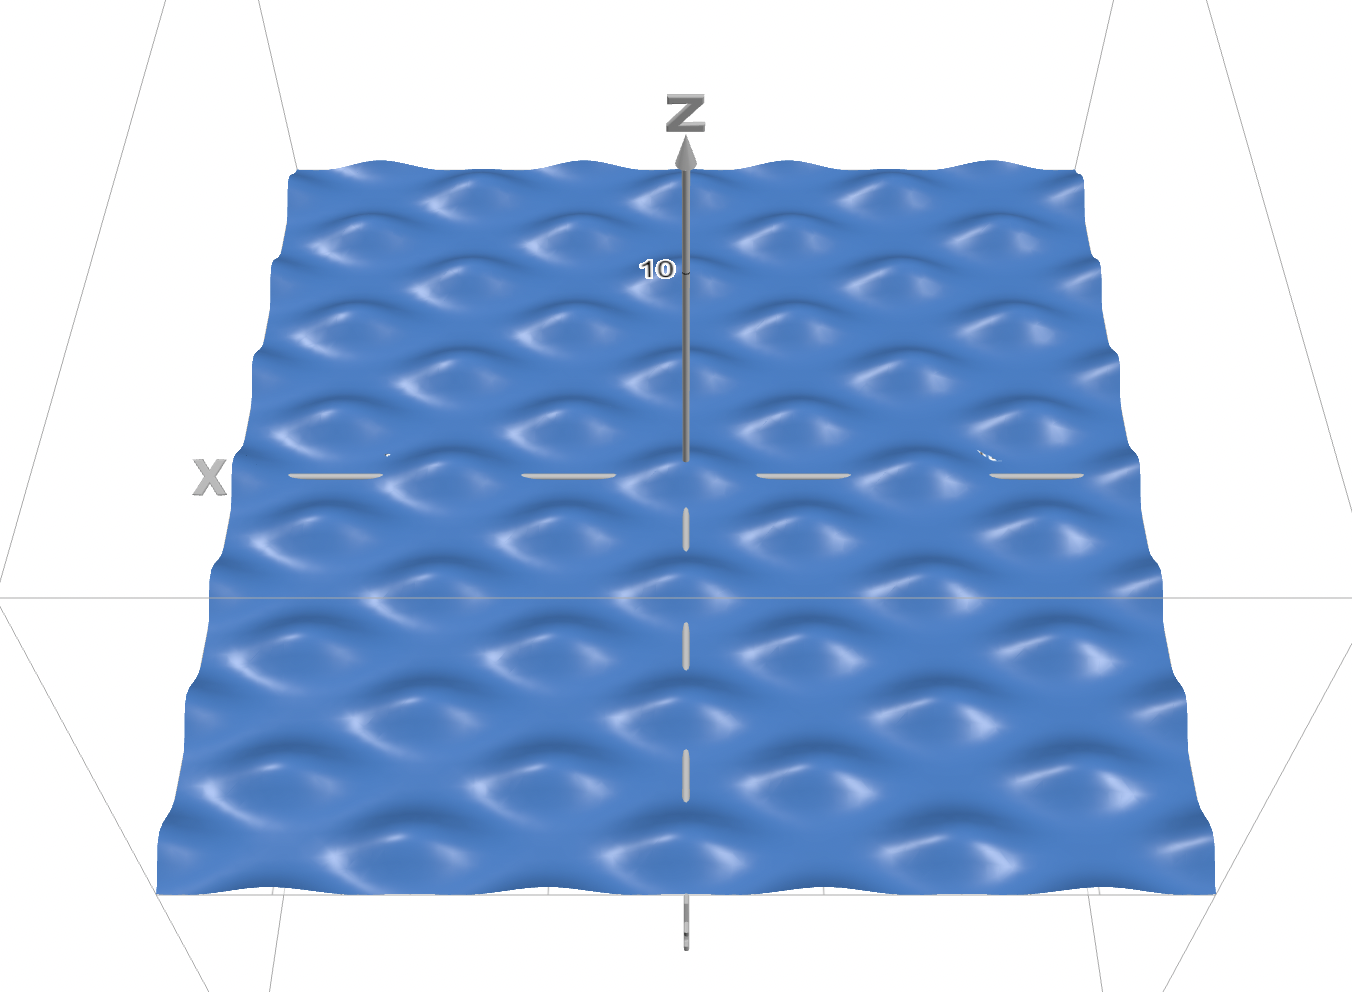
\includegraphics[width=0.7\textwidth]{hex grid.png}\label{fig:hex grid}\caption{A plot of the term in the hp objective function that ``encourages'' vertices to grid points: $\left[\cos(
        \frac{\pi}{\sigma}(u_{i_y}+\frac{u_{i_x}}{\sqrt{3}})
    ) \cos(
        \frac{\pi}{\sigma}(u_{i_y}-\frac{u_{i_x}}{\sqrt{3}})
    )\right]^2$}
\end{figure}

\subsection{22.5}
Theoretically, there may be an objective function that moves vertices to ``nice'' 22.5 locations (for example, $x$ and $y$ coordinates in the form of $\frac{a+b\sqrt2}{c}$ where $a$ and $b$ are low and $c$ is a power of 2). It's also likely ok to change the flap lengths within some tolerance, since the user will likely be inputting flap lengths as rational numbers while most flap lengths will end up as something in the form of $\frac{a+b\sqrt2}{c}$.

\section{Design pipeline}
The dream is a software that given a tree (perhaps with additional conditions like symmetry or specific nodes fixed to the paper edge), will be able to spit out a full crease pattern to be folded in bp, hp, or 22.5. I propose something like the following:

First, run the tree some $N$ times with randomized initial positions using the circle packing constraint (\ref{eq:circle}) and objective function $-\sigma$. Generally a good solution in bp/hp/22.5 will be close to a good solution in circle packing, and running multiple times with circle packing (the computationally easiest) increases the chances of finding better local optima. 

Then, for each of the best $n$ unique results, use the circle packed positions as initial positions for the bp/hp/22.5 solver. Run the solver with the corresponding constraint equations and objective functions. Finally, display the options for the user to choose from. (Note: then constructing the cp will be a whole other issue, mainly because there may be empty space to fill.)

\section{Preliminary results}
Below are the best 6 out of a runs of 70 solutions each, first generated with circle packing and then converting the best results into the respective bp, hp, and 22.5. All used a tree with four flaps of length 3, three flaps of length 6, and two flaps of length 9. Hyperparameters are: $\alpha=100$, $C_1=1$, $C_2=1$, $b=0.2$, and $k=1$. The solver is written in python, using the scipy library. Runtimes were within 20s for each of the 4 runs.

\begin{figure}
    \centering
    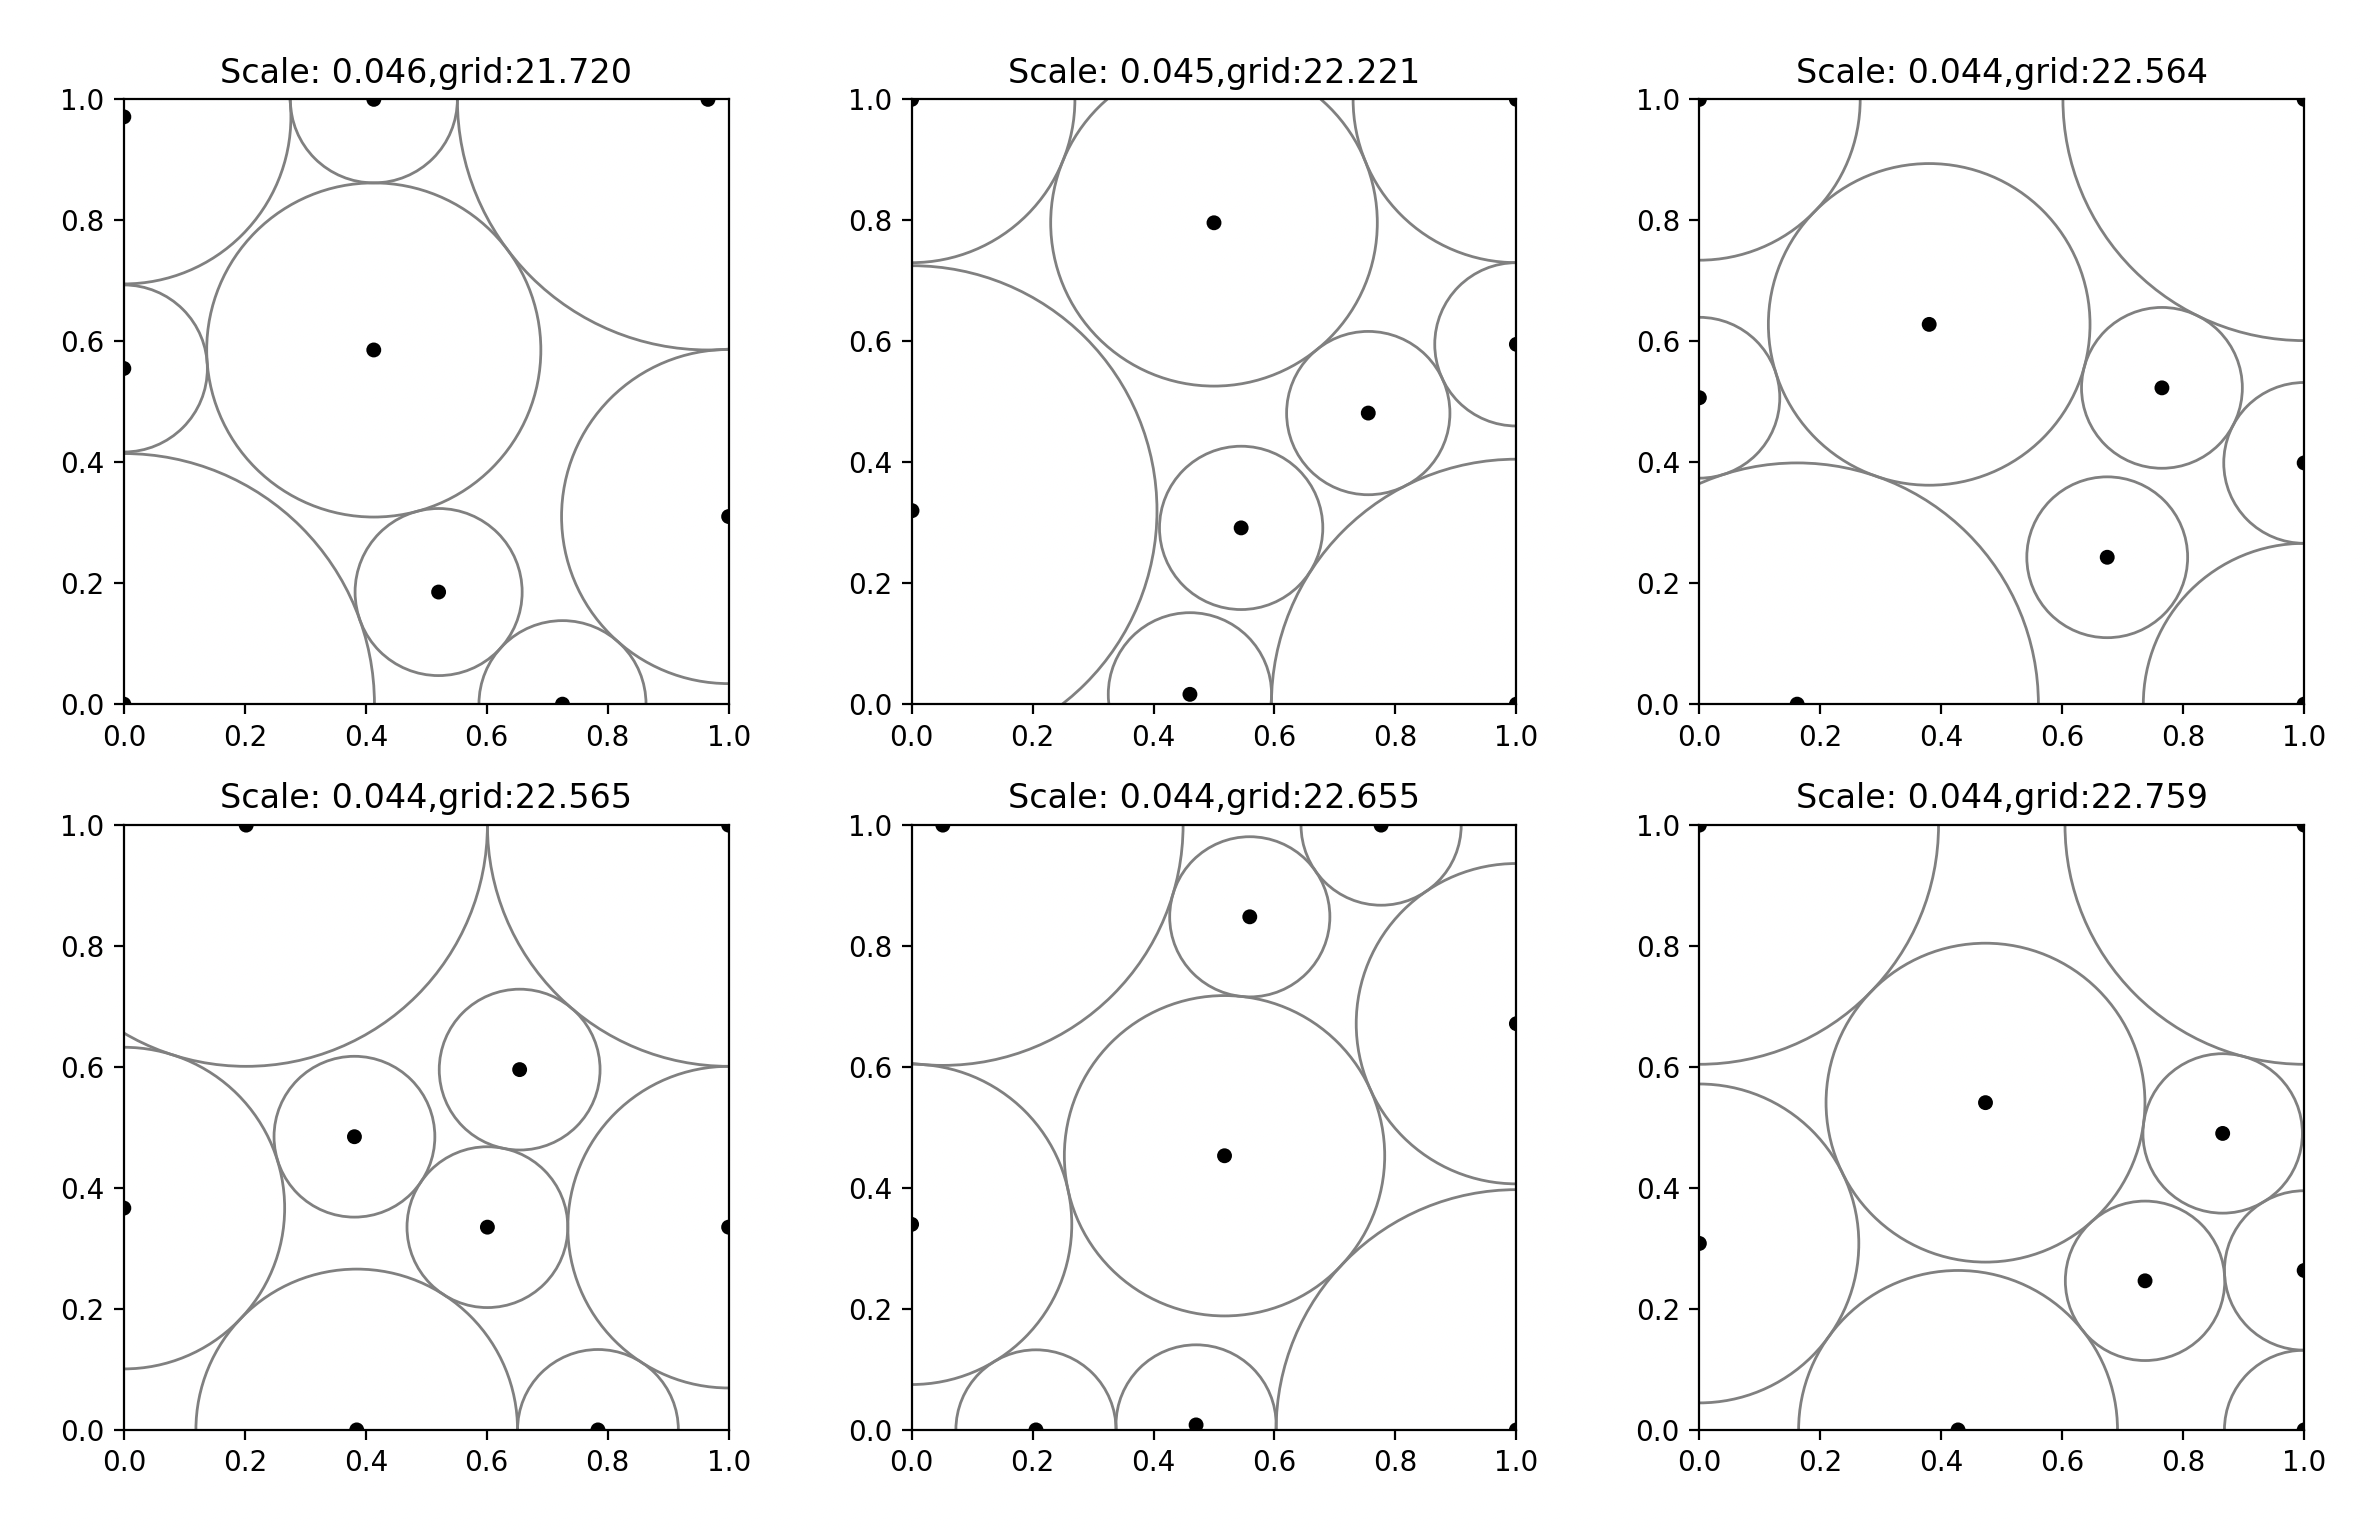
\includegraphics[width=0.9\textwidth]{circle packings2.png}\label{fig:circles}\caption{Some circle packing solutions}
\end{figure}
\begin{figure}
    \centering
    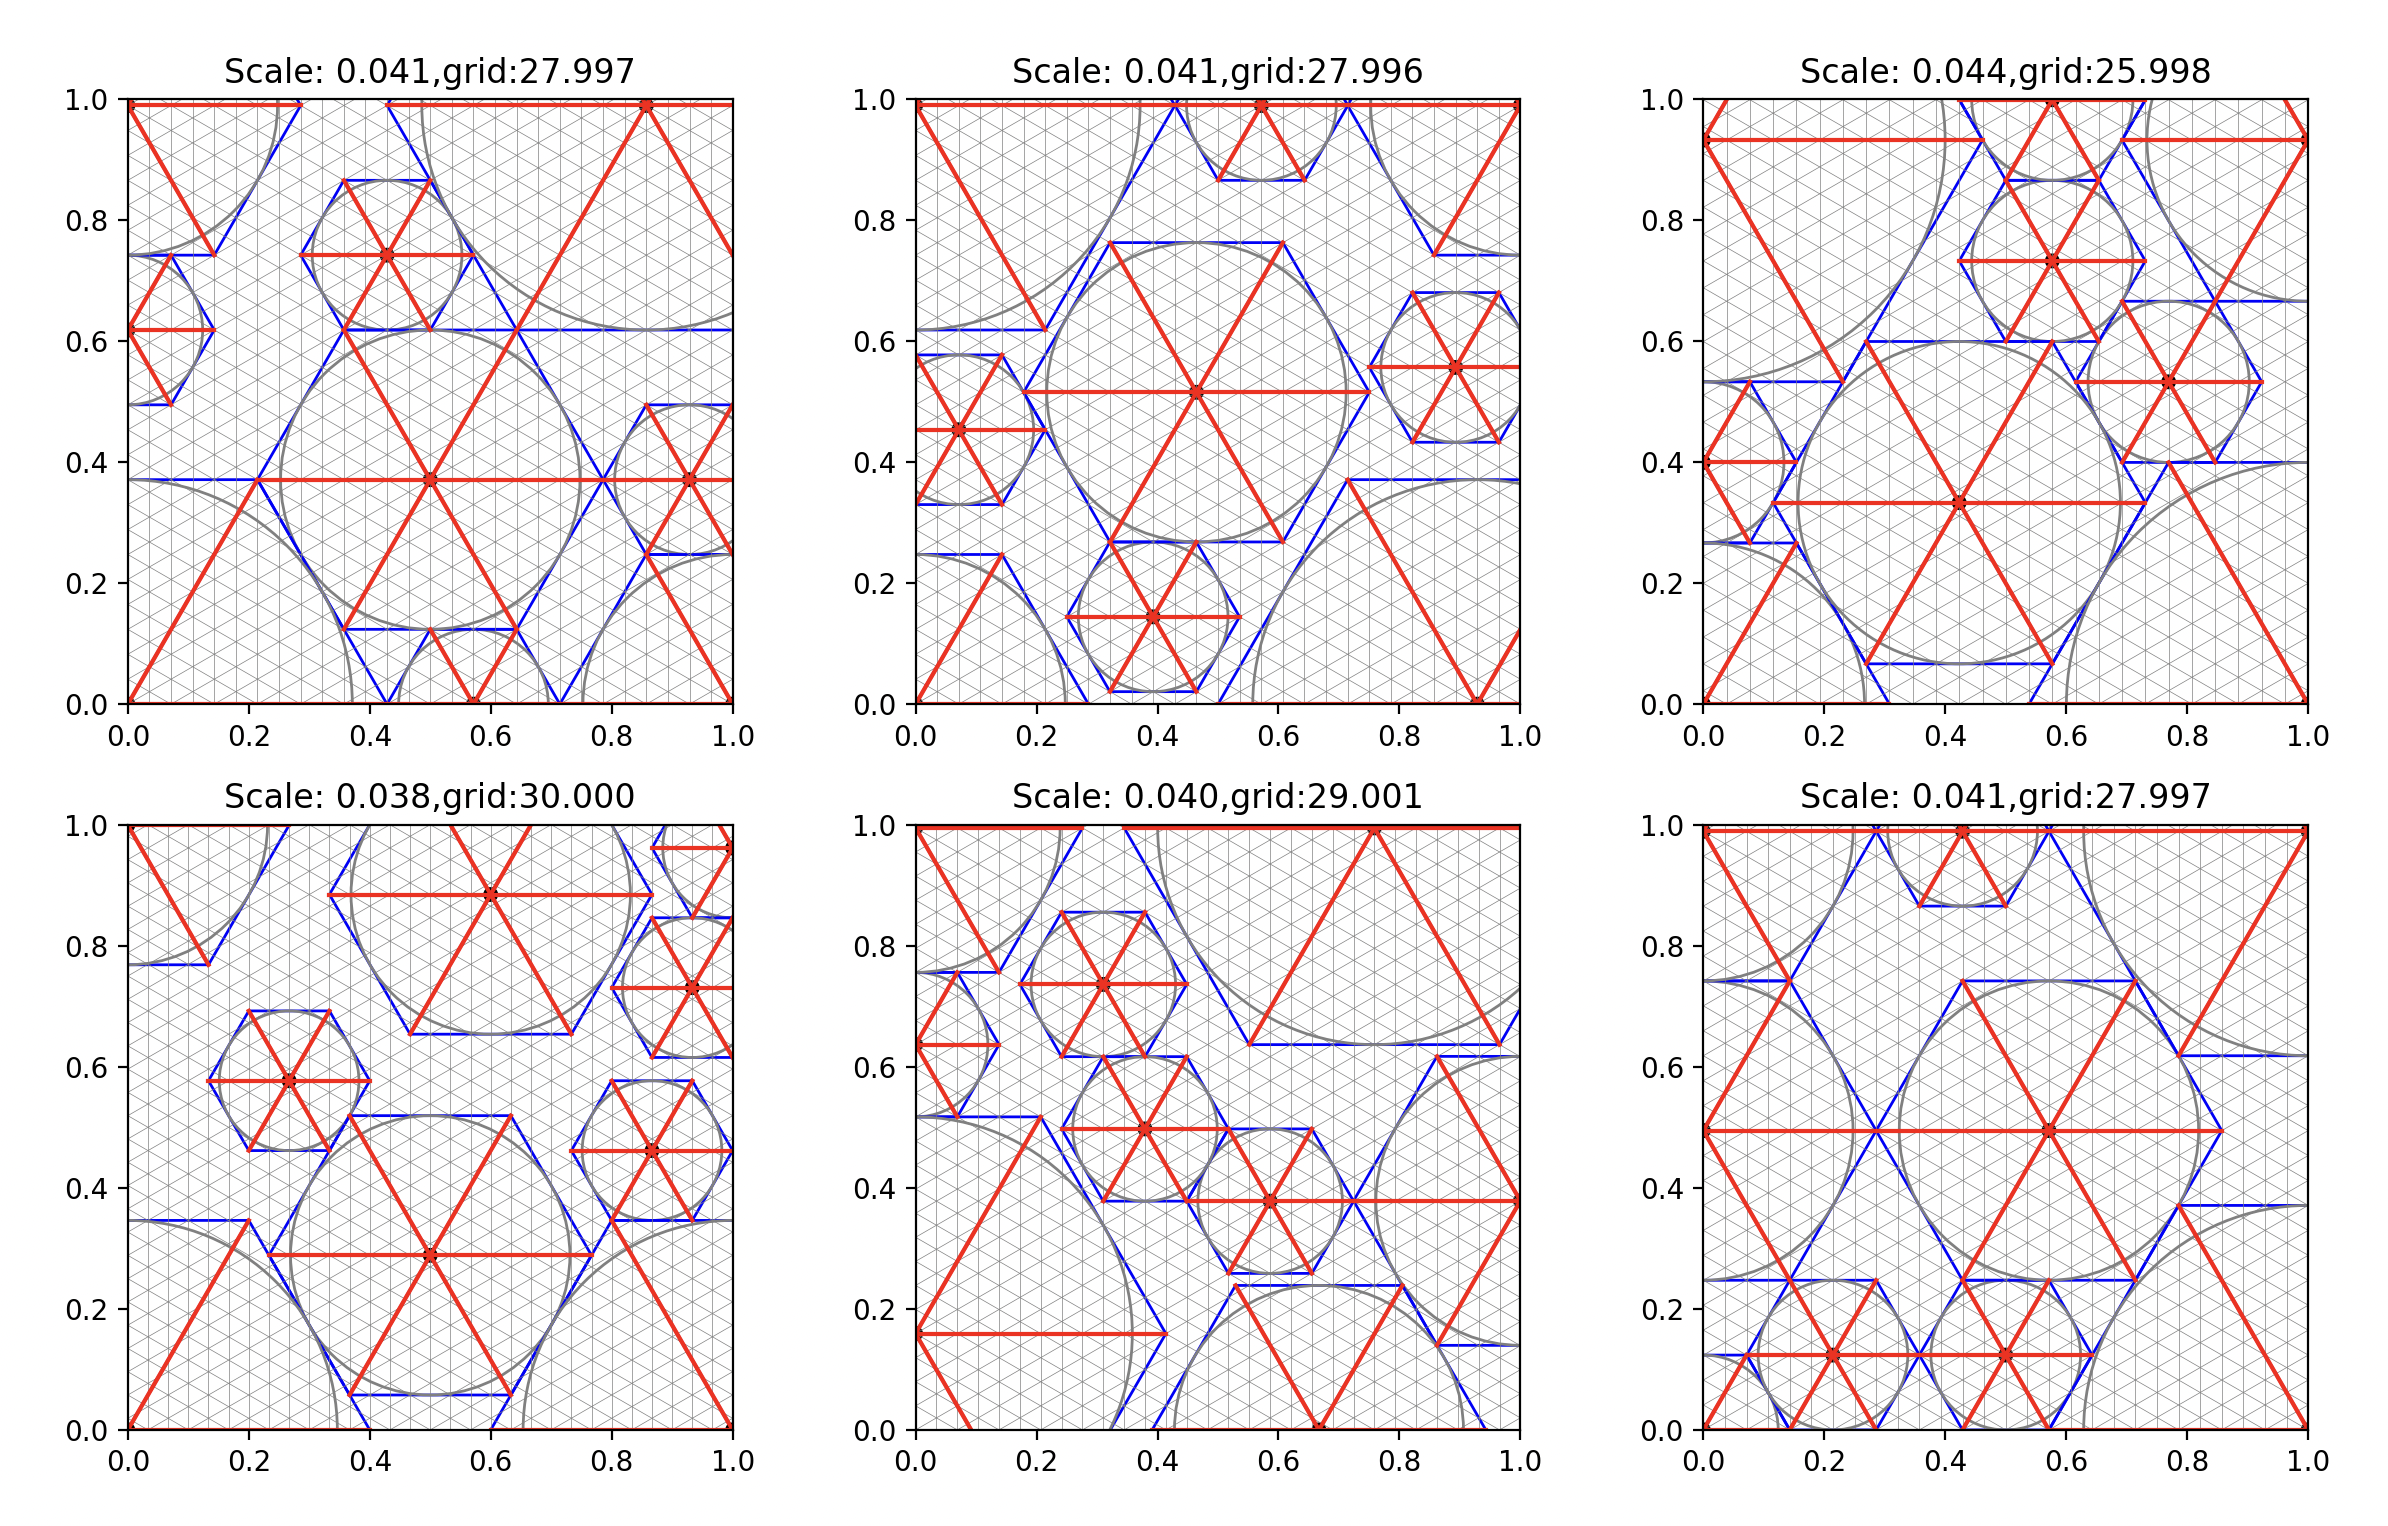
\includegraphics[width=0.9\textwidth]{hex packings 2.png}\label{fig:hexagons}\caption{Some hex packing solutions.}
\end{figure}
\begin{figure}
    \centering
    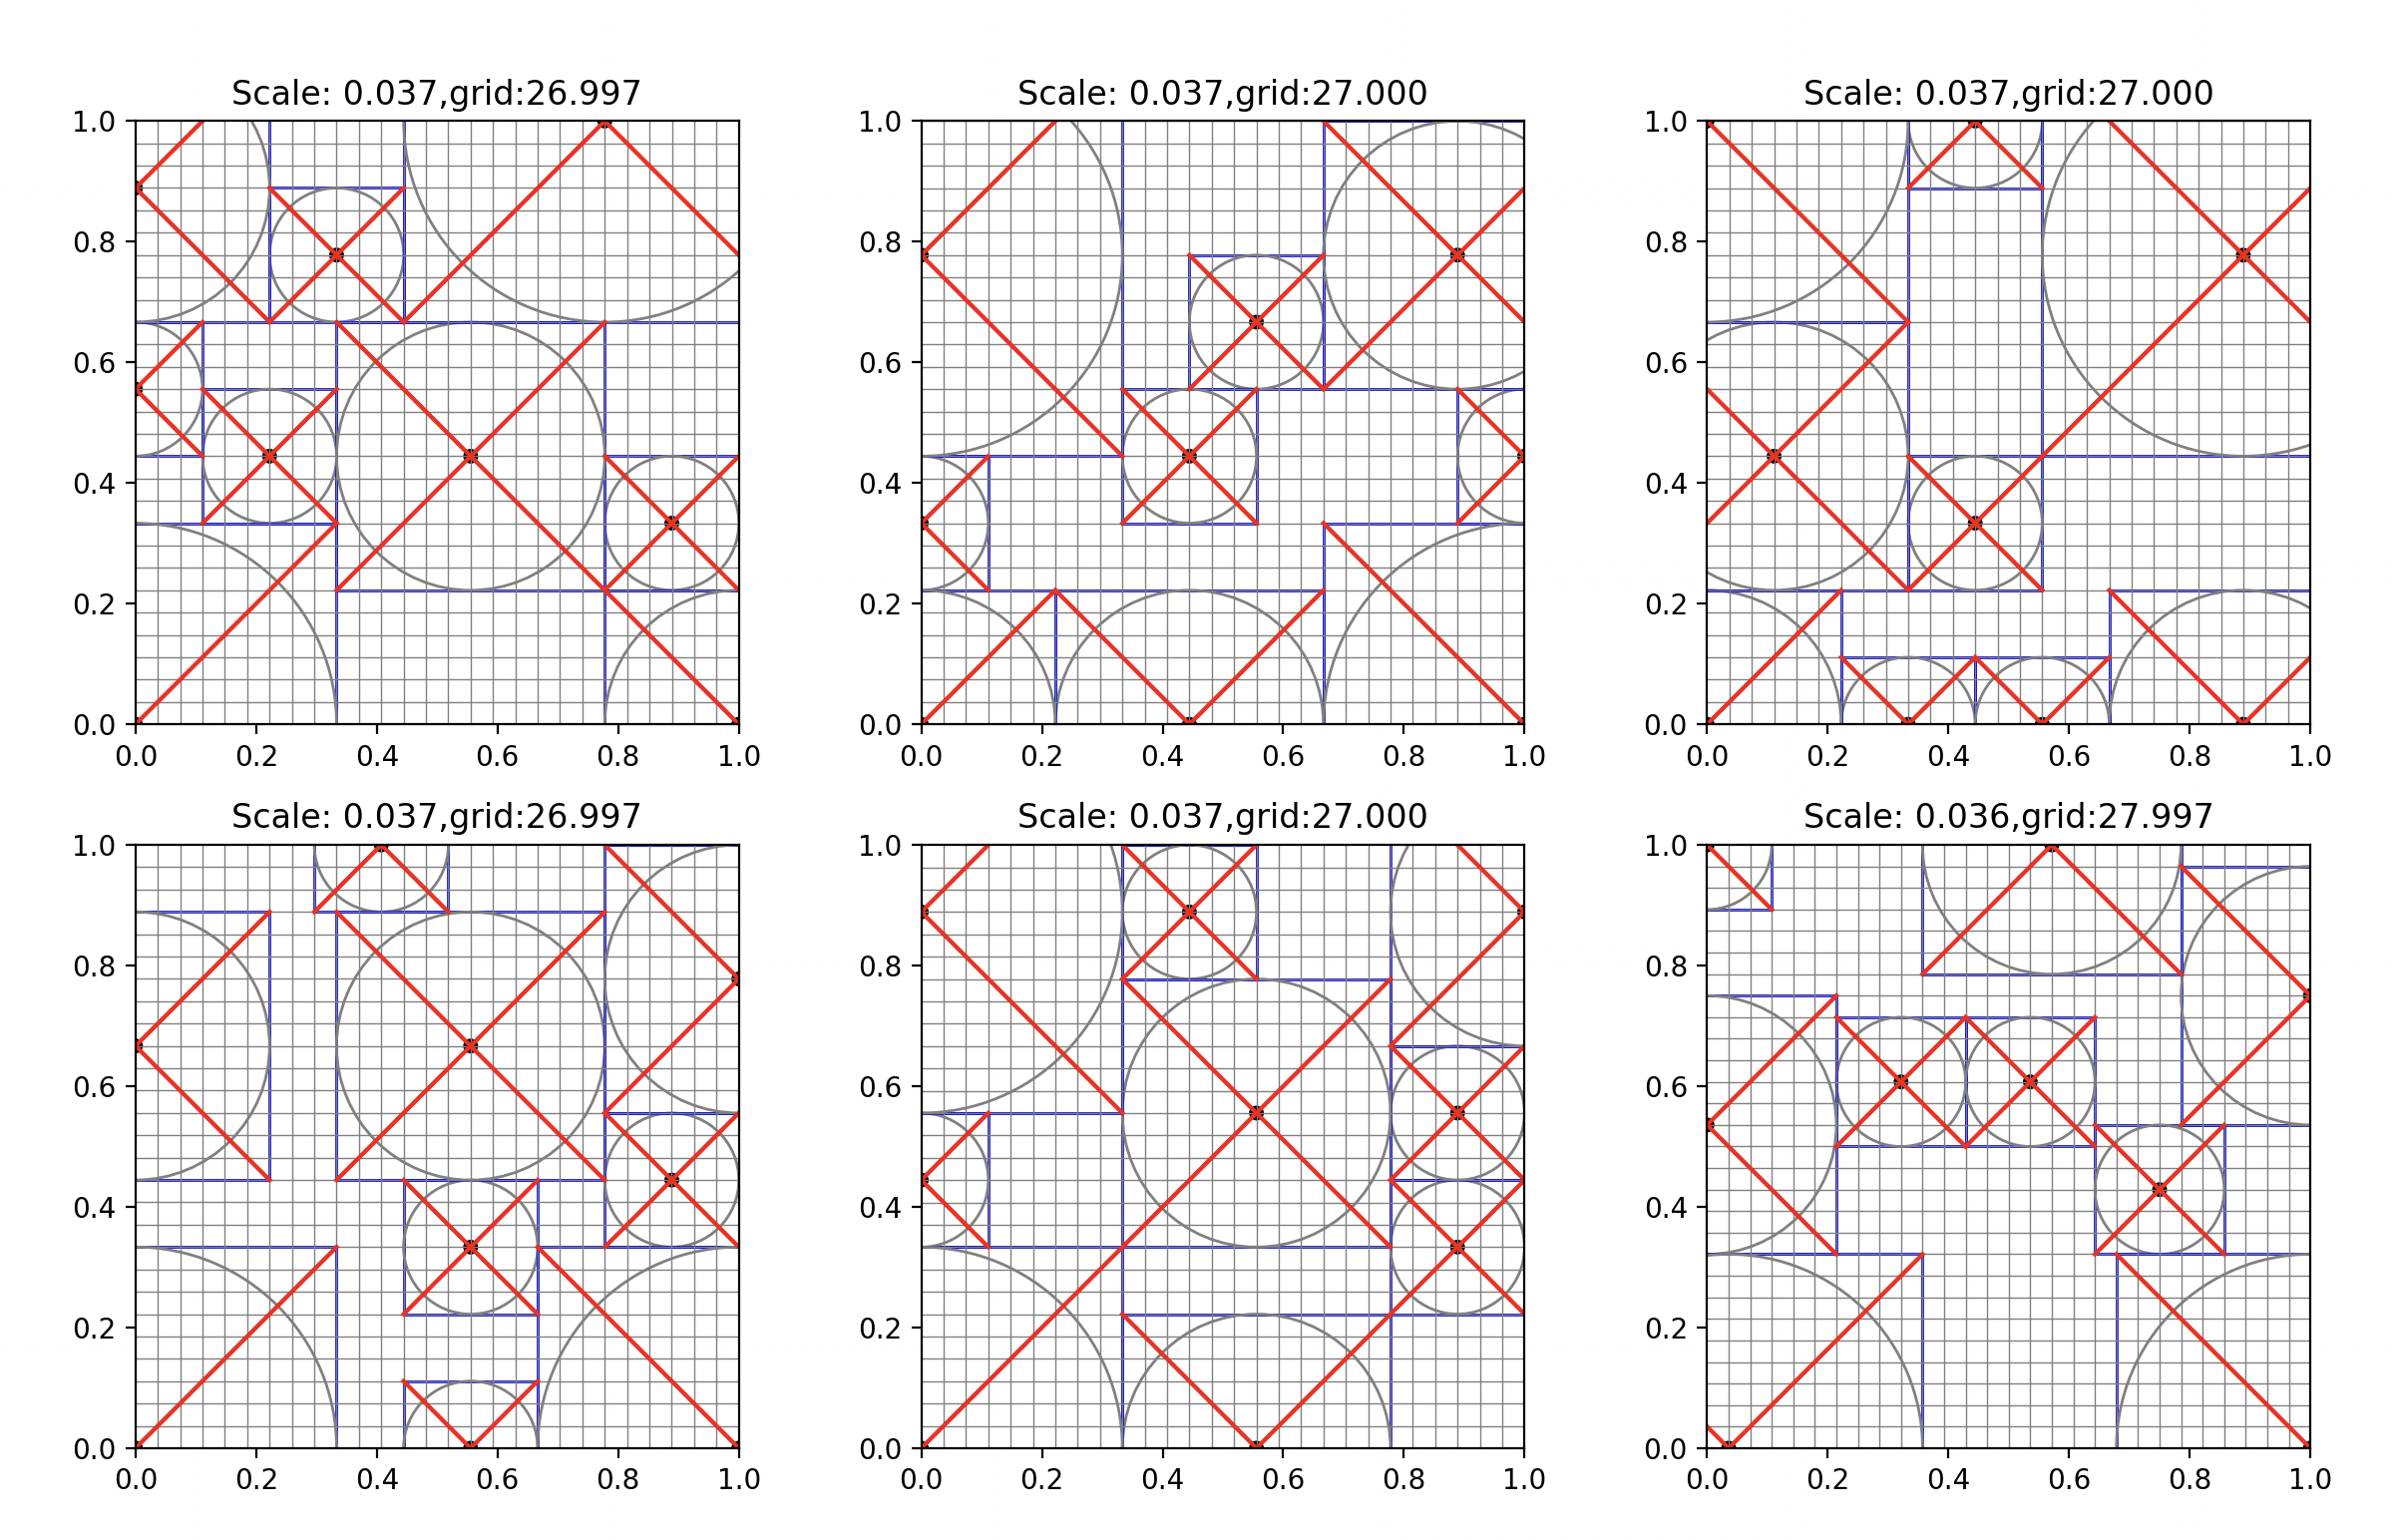
\includegraphics[width=0.9\textwidth]{square packings 2.png}\label{fig:squares}\caption{Some square packing solutions}
\end{figure}
\begin{figure}
    \centering
    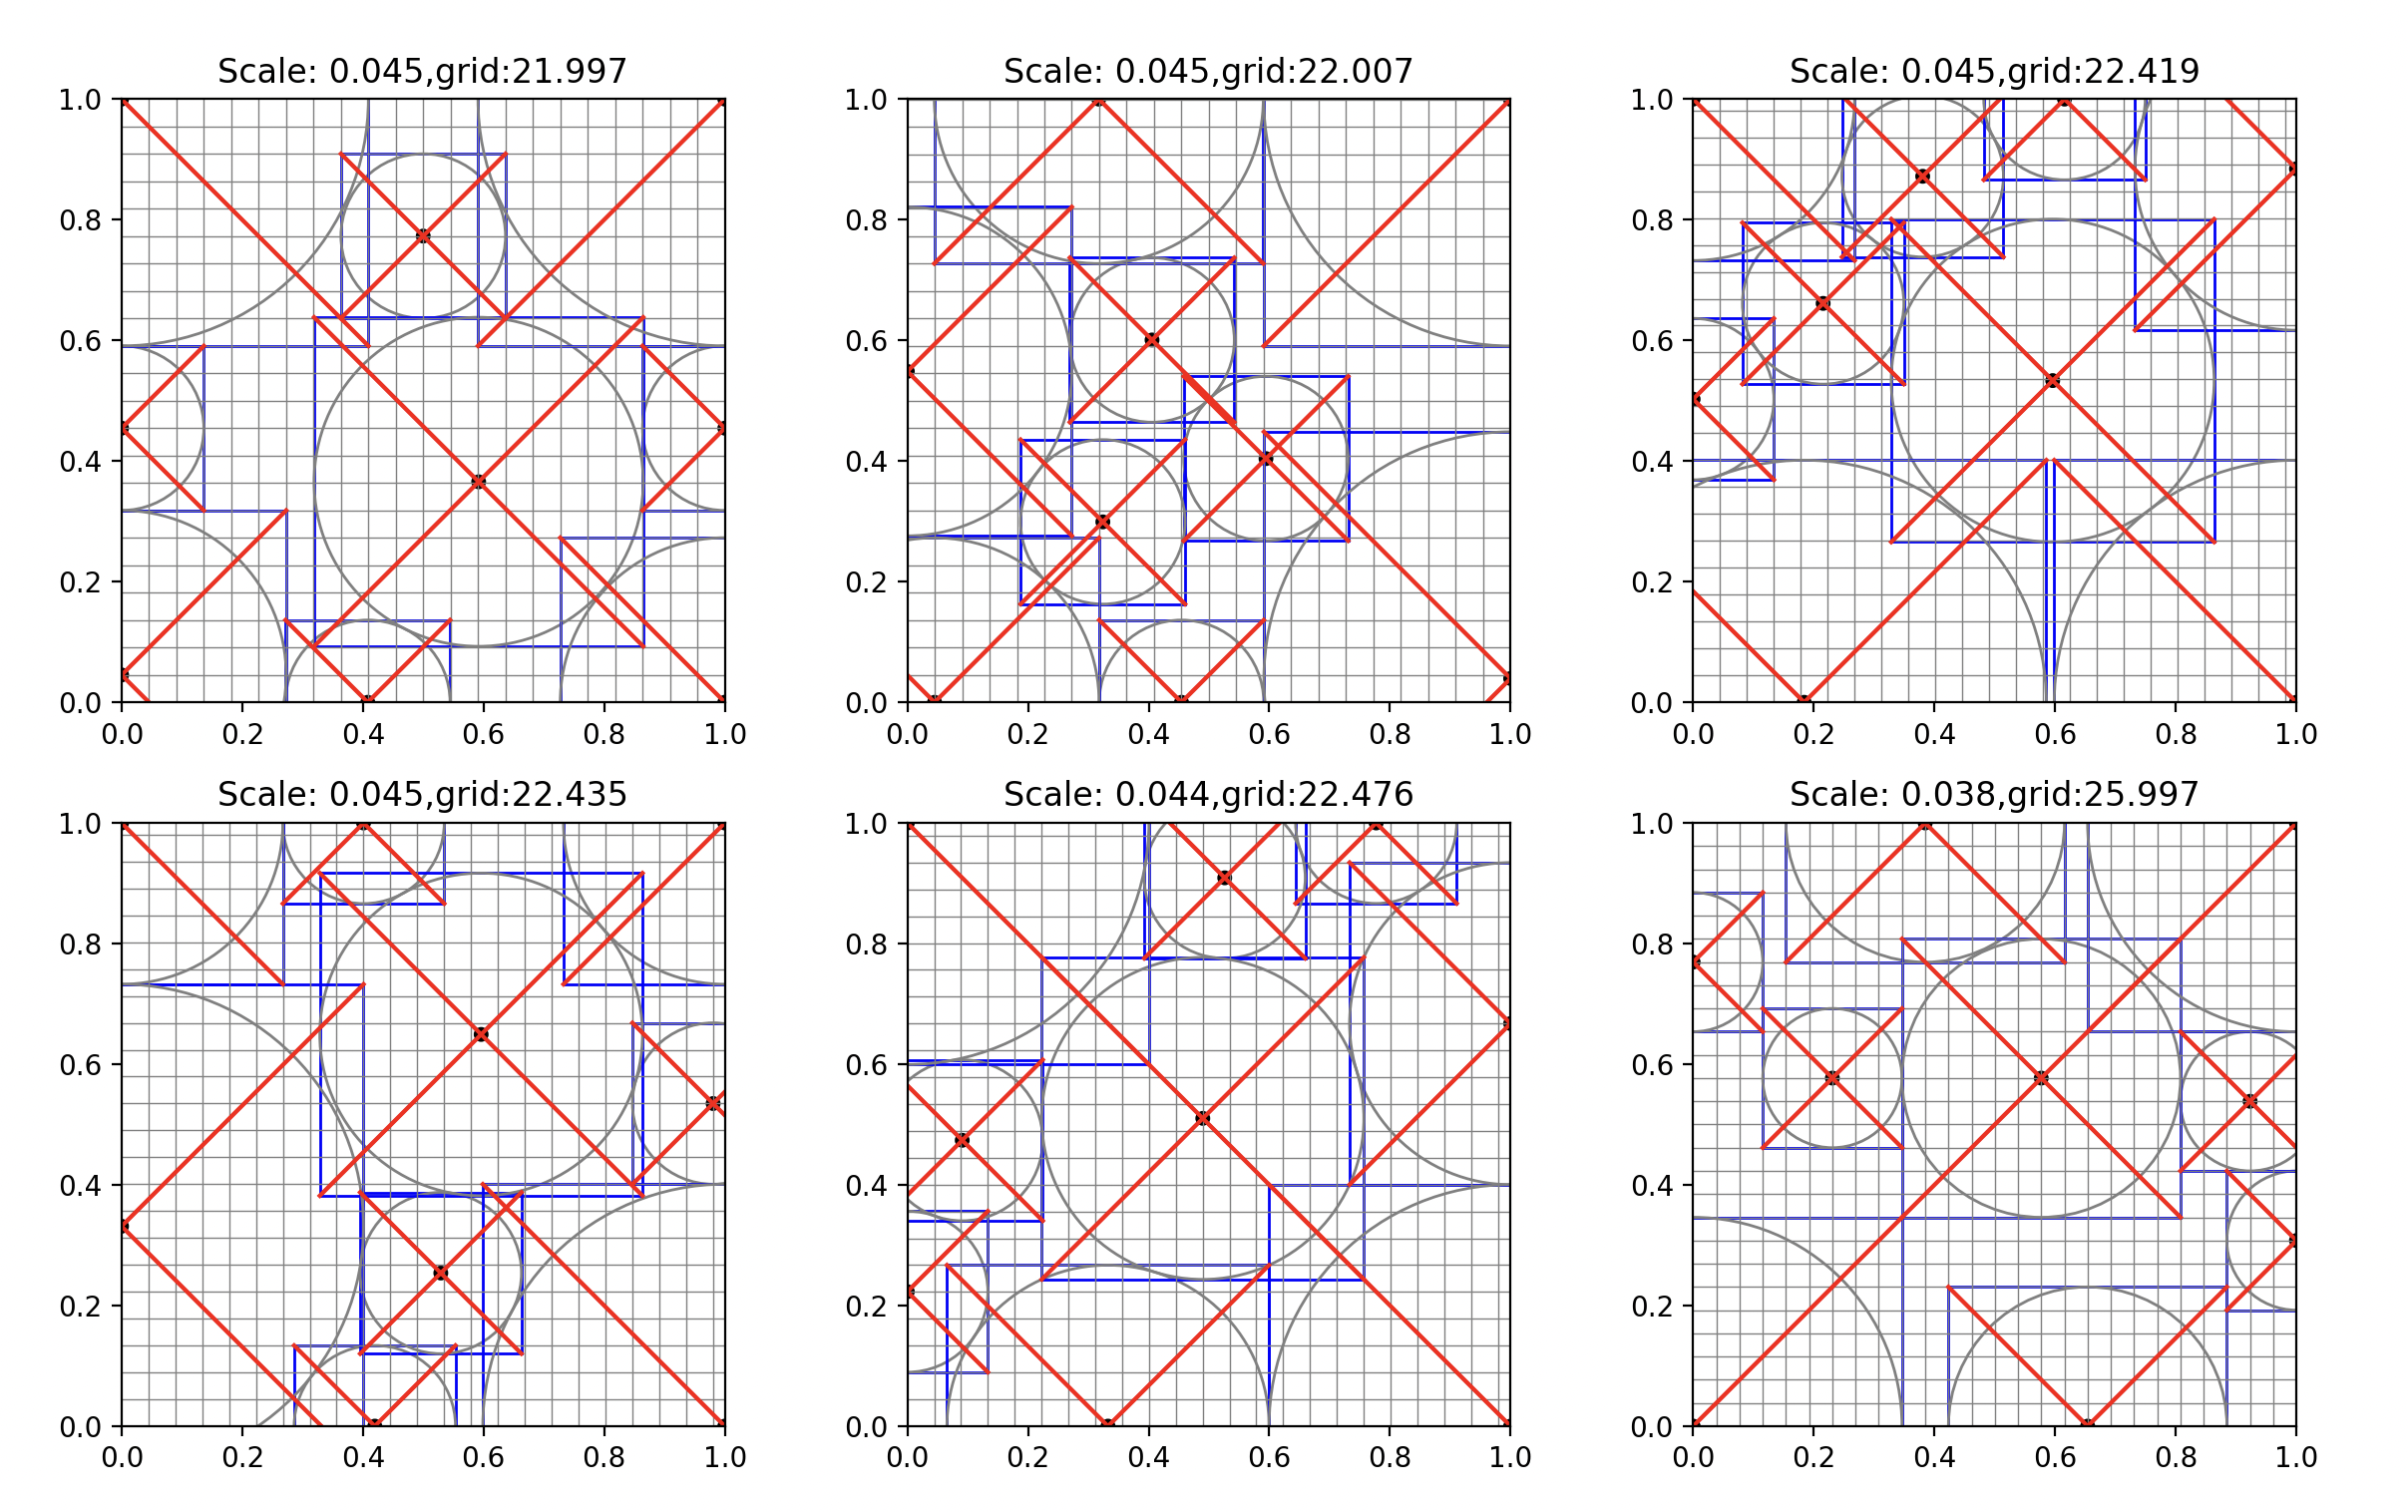
\includegraphics[width=0.9\textwidth]{square packings pythas.png}\label{fig:squares pythas}\caption{Some square packing solutions that allow pythagorean stretches. Some solutions have off-grid vertices, but a few don't.}
\end{figure}

\begin{figure}
    \centering
    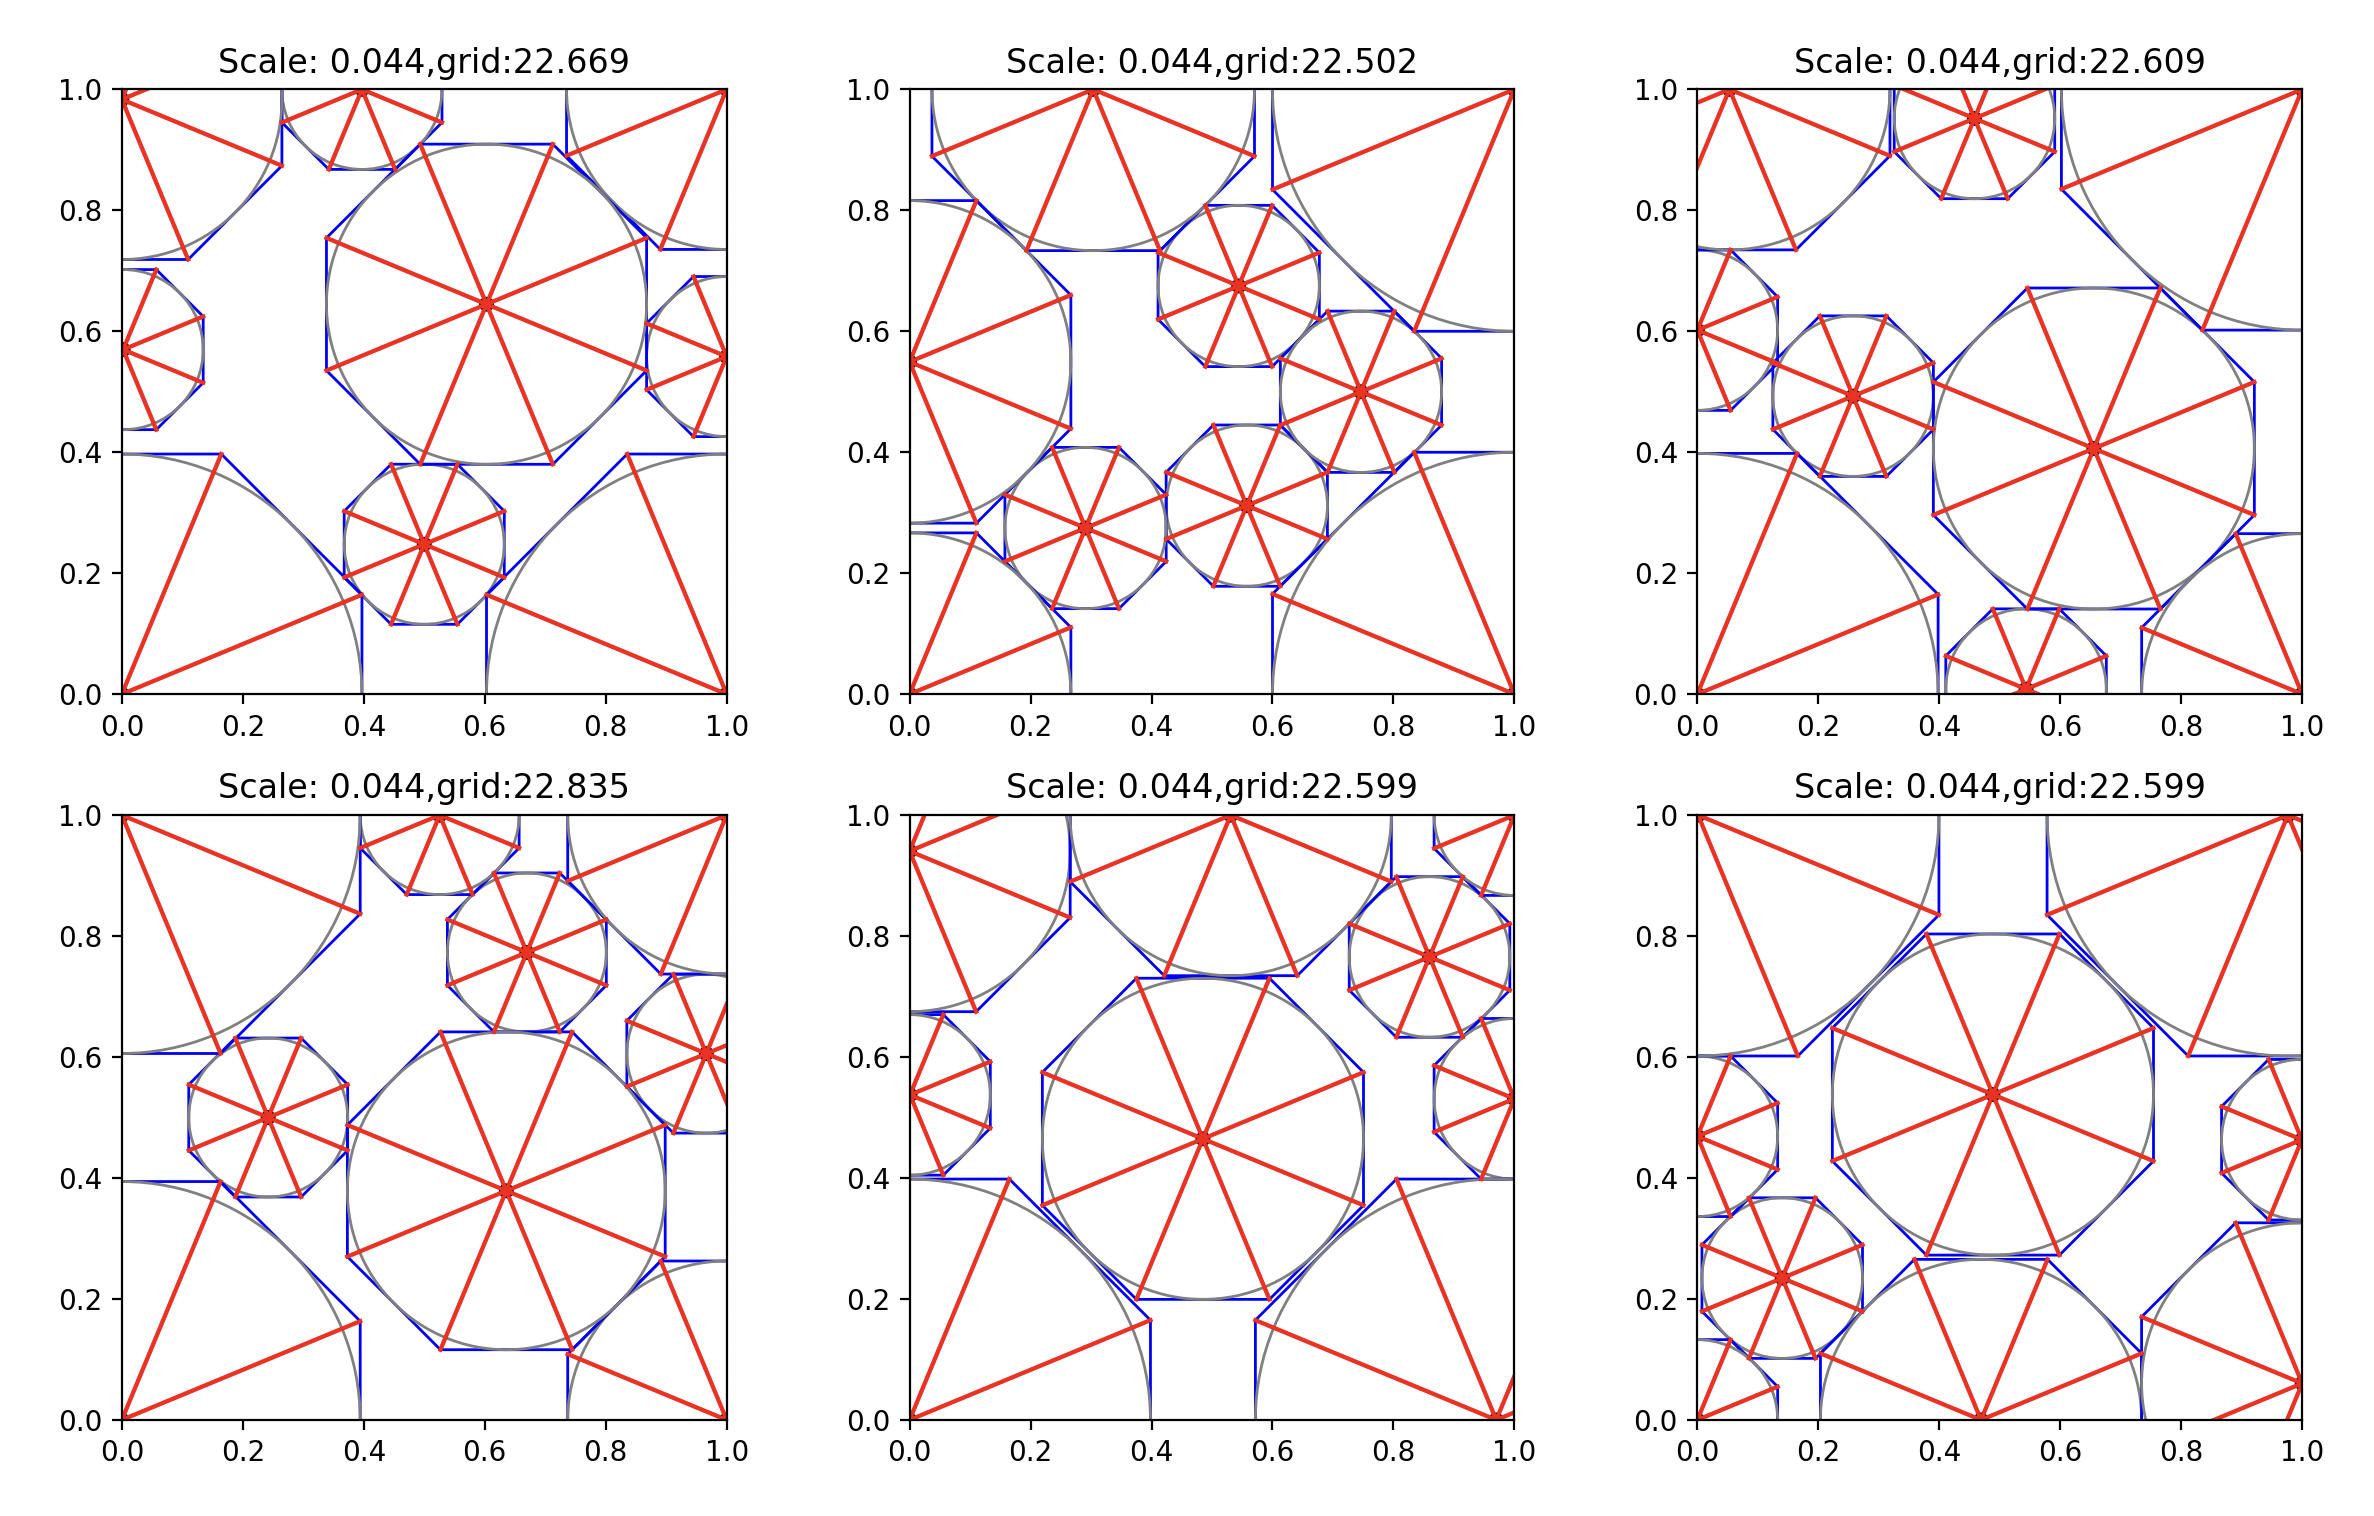
\includegraphics[width=0.9\textwidth]{octagon packings 2.png}\label{fig:octagon packings}\caption{Some octagon packing solutions using the standard octagon packing constraint.}
\end{figure}
\begin{figure}
    \centering
    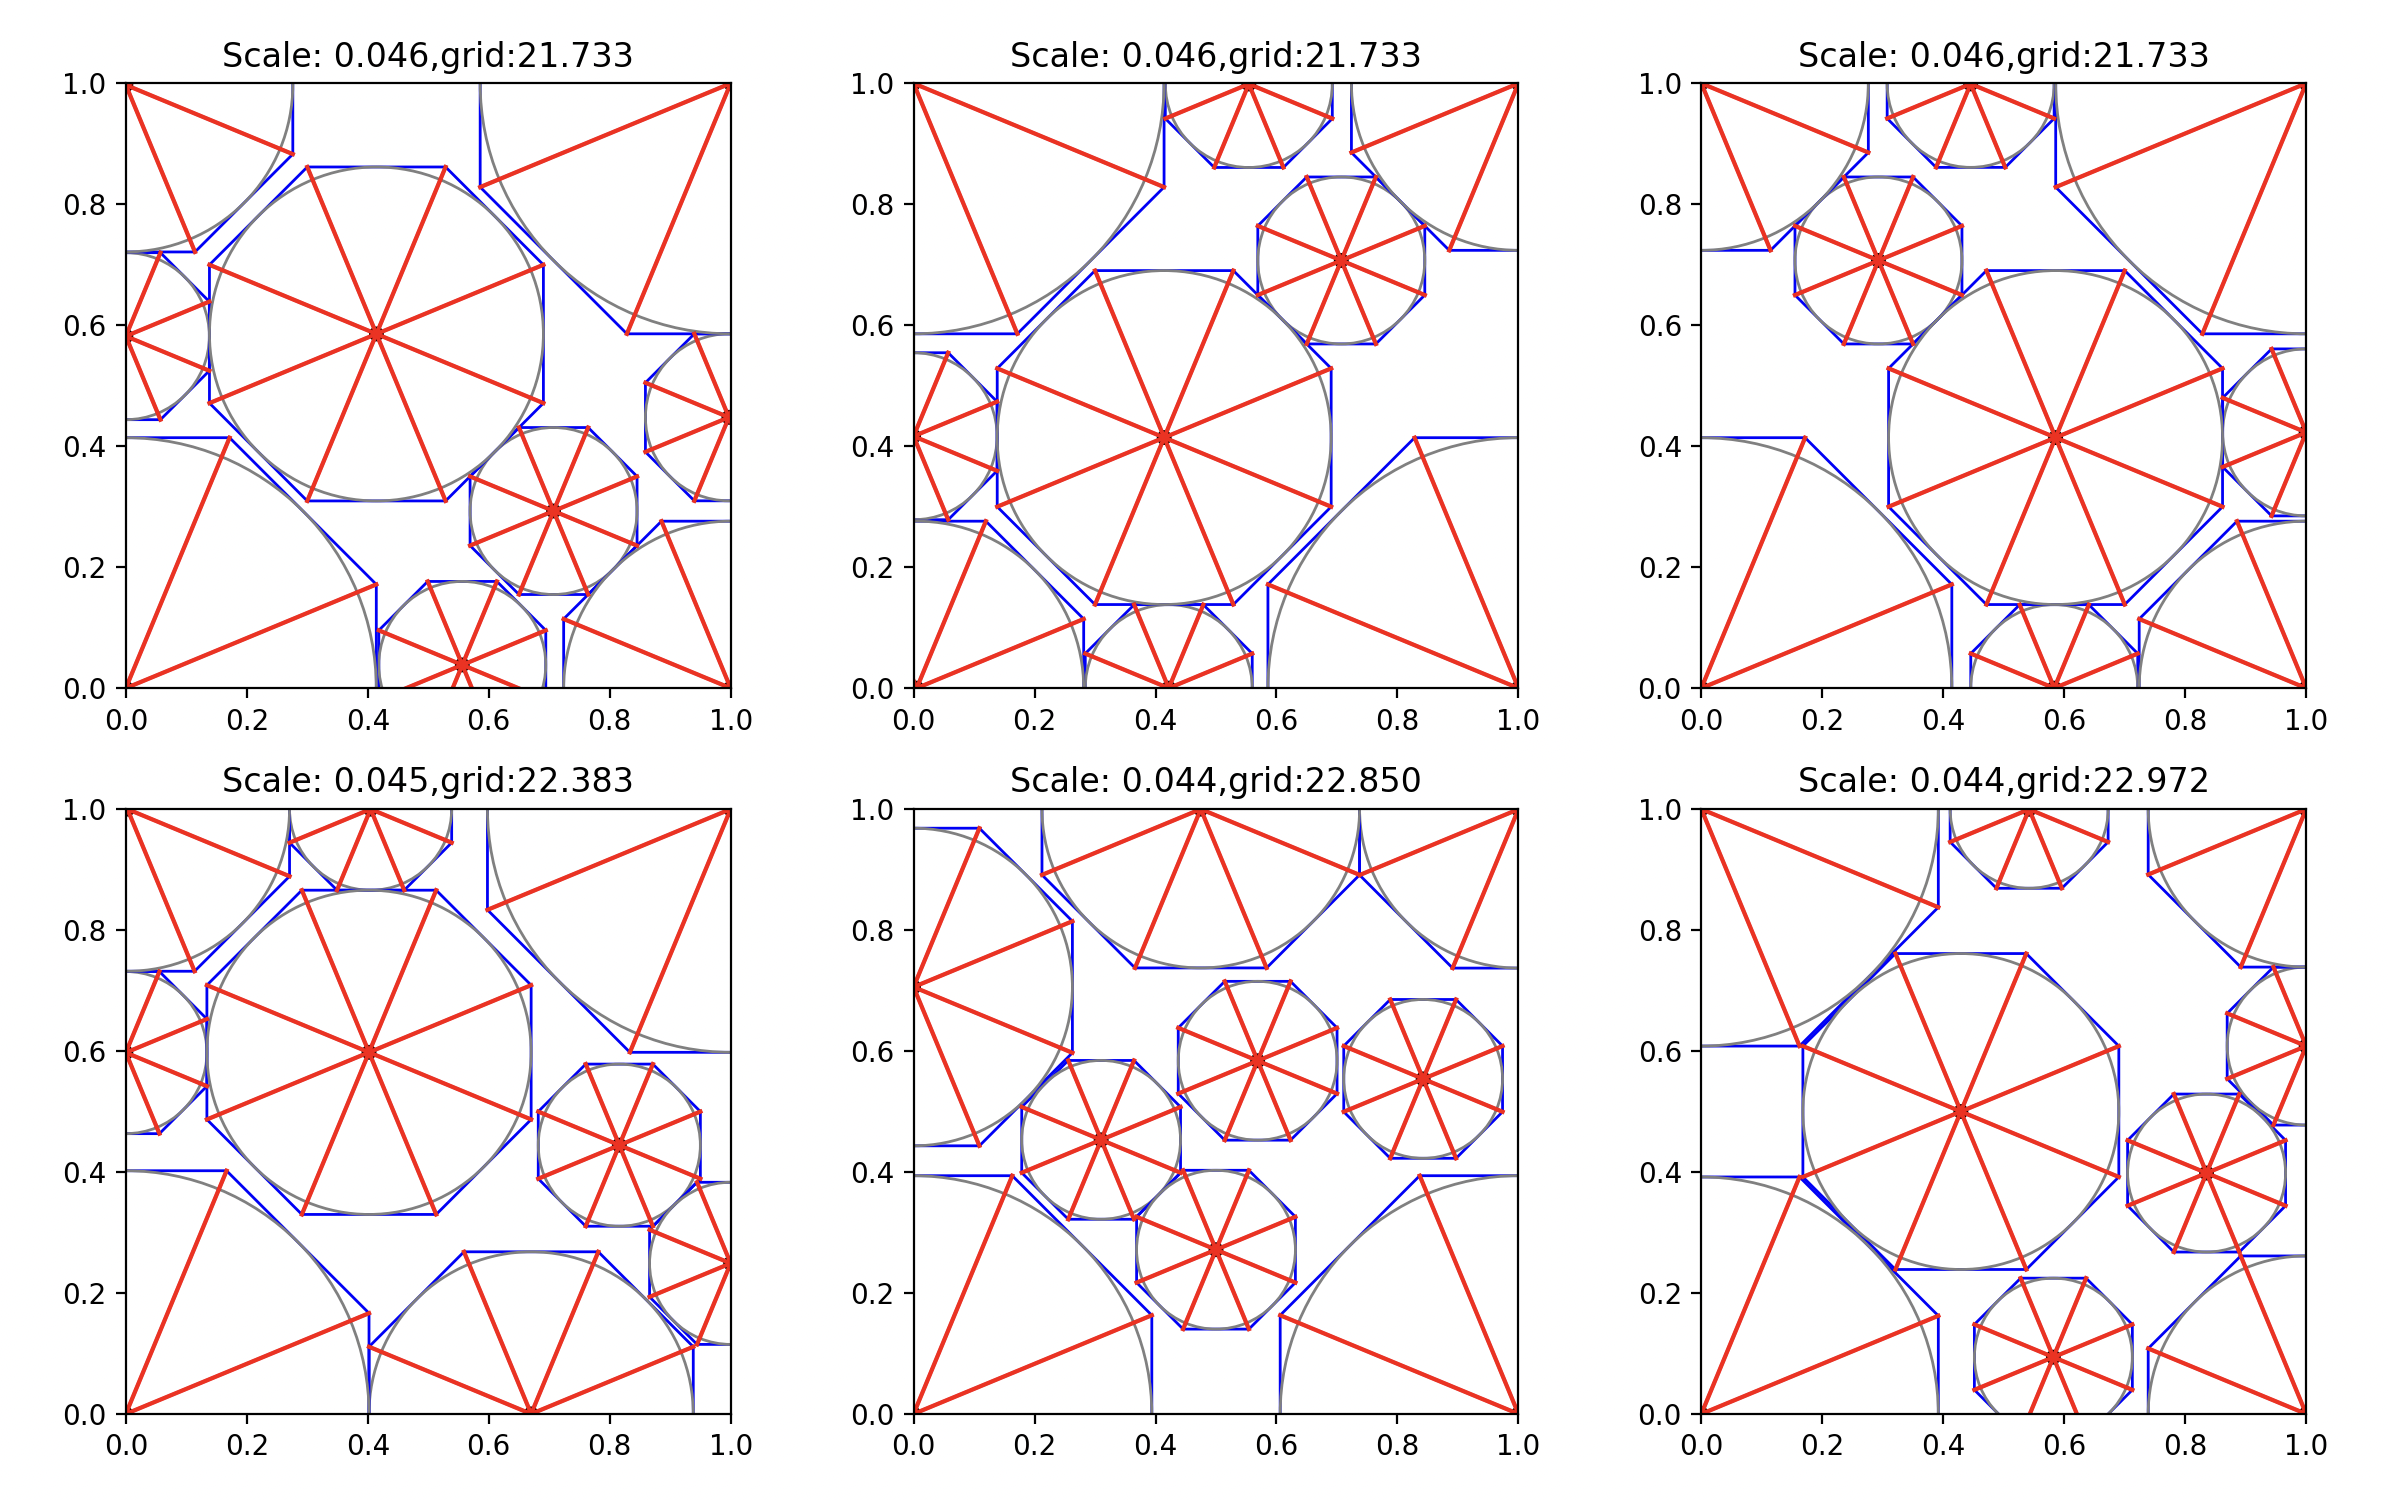
\includegraphics[width=0.9\textwidth]{octagon packings polar.png}\label{fig:octagon packings polar}\caption{Some octagon packing solutions using the polar constraint (\ref{eq:polar}) with $b=0.1$ and $k=1$ to encourage active paths to lie on 45 degree axial lines.}
\end{figure}

% --------------------------------------------------------------
%     You don't have to mess with anything below this line.
% --------------------------------------------------------------
 
\end{document}